\documentclass[12pt,a4paper,ngerman]{report}
\usepackage{babel}
%\usepackage{natbib}
\usepackage{url}
%\usepackage[left=2cm, right=1.5cm, top=2cm, bottom=2cm]{geometry}
%\usepackage[ansinew]{inputenc}
\usepackage{amsmath}
\usepackage{nicefrac} % macht schöne Brüche mit querstrich mit \nicefrac{1}{2}
\usepackage{graphicx}
%\graphicspath{}
\usepackage{titlesec}% um chapterüberschriften anzupassen.
\titleformat{\chapter}{\normalfont\huge\bf}{\thechapter.}{20pt}{\huge\bf}
\usepackage{parskip}
\usepackage{fancyhdr}
\usepackage{amsfonts}
\usepackage{float}
\usepackage{caption}
\usepackage{subcaption} % for \begin{subfigure}
	
\usepackage{csquotes} % mit \enquote{blabla} tolle anfürungsstriche erstellen
%\usepackage{physics} %lässt mich \bra und \ket benuzen %im konflict mit siunitx
\usepackage{amssymb} % für \gtrsim und \lesssim

\usepackage{pgfplots} %für plots
\pgfplotsset{compat=newest}

\usepackage{varioref} % macht mit \vref{} viel bessere referenzen
\usepackage{hyperref} % macht klickbare referenzen

\usepackage{xcolor, soul} %mit \hl{} kann man toll Sachen hervorheben.
\newcommand{\highlight}[1]{%
	\colorbox{yellow!50}{$\displaystyle#1$}} % mit \highlight{} kann man sogar in Gleichungen hervorheben

\usepackage{vmargin}
\usepackage[section]{placeins}
\usepackage{capt-of}
\usepackage{enumitem}
\usepackage{multirow}
\usepackage{blindtext}
\usepackage{lipsum}
\usepackage[version=4]{mhchem} % um Chemische Elementsymbole zu benutzen: \ce{H20}

\usepackage{pdfpages} % um PDFs einzufügen

%spread to latex:
\usepackage{booktabs, multirow} % for borders and merged ranges
\usepackage{changepage,threeparttable} % for wide tables

\providecommand{\e}[1]{\ensuremath{\cdot 10^{#1}}}
\providecommand{\fehlt}{\textcolor{red}{{ ¡Fehlt! }}}
\providecommand{\mytitle}{Plasmakristall}

\usepackage{siunitx}
\sisetup{
	separate-uncertainty = true,
	%per-mode = fraction,
	%per-mode = symbol
}
\DeclareSIUnit\bar{bar}
\DeclareSIUnit\atomicmassunit{u}
\usepackage{isotope}


\setmarginsrb{3 cm}{2.5 cm}{3 cm}{2.5 cm}{1 cm}{1.5 cm}{1 cm}{1.5 cm}
\title{\mytitle} % Title


\author{Frederik Uhlemann, Florian Adamczyk}
% Author
\date{\today}
% Date

\makeatletter
\let\thetitle\@title
\let\theauthor\@author
\let\thedate\@date
\makeatother

\pagestyle{fancy}
\fancyhf{}
\rhead{\theauthor}
\lhead{\mytitle}
\cfoot{\thepage}
%%%%%%%%%%%%%%%%%%%%%%%%%%%%%%%%%%%%%%%%%%%%
\begin{document}
		
	%%%%%%%%%%%%%%%%%%%%%%%%%%%%%%%%%%%%%%%%%%%%%%%%%%%%%%%%%%%%%%%%%%%%%%%%%%%%%%%%%%%%%%%%%
	
	\begin{titlepage}
		\centering
		\vspace*{0.5 cm}
		% \begin{large} Justus-Liebig-Universität\\ Gießen \end{large}
		
\includegraphics[width = 0.6 \textwidth]{JLU_Giessen-Logo}	%University Logo
		\\[2.0 cm]
		% \begin{center}    \textsc{\Large Justus - Liebig - Universität}\\{Giessen}\\[0.8cm]	\end{center}% University Name
		Versuch 7 des\\
		\textsc{\Large Fortgeschrittenen-Praktikums}\\ [0.3 cm]				% Course Code
		\rule{\linewidth}{0.2 mm} \\[0.4 cm]
		{ \huge \bfseries \thetitle}\\
		\rule{\linewidth}{0.2 mm}\\
		Versuchstermin 22.07.2024 \\
		~ \\
		[2.0 cm]
		
		
		\begin{minipage}{0.49\textwidth}
			\begin{flushleft}
				 \emph{Praktikumsbetreuer:}\\
				 Michael Kretschmer\\
				 %  Affiliation\\
				 \small{\href{mailto:michael.kretschmer@exp1.physik.uni-giessen.de}{michael.kretschmer@exp1.physik.uni-giessen.de}}
			\end{flushleft}
		\end{minipage}~
		\begin{minipage}{0.49\textwidth}
			\begin{flushright}
				\emph{Protokoll von:} \\
				
				\large{Frederik Uhlemann}\\
				\small{\href{mailto:frederik-vincent.uhlemann@physik.uni-giessen.de}{frederik-vincent.uhlemann@physik.uni-giessen.de}\\~\\
					%Matrikel Nr.: \:  \\[0.5cm]
					%\href{mailto:}{}
				}
				\large{Florian Adamczyk} \\
				\small{\href{mailto:florian.marius.adamczyk@physik.uni-giessen.de}{florian.marius.adamczyk@physik.uni-giessen.de}\\
					%Matrikel Nr.: \: 8105234}
			}
		\end{flushright}
	\end{minipage}
	
	\end{titlepage}
	
%%%%%%%%%%%%%%%%%%%%%%%%%%%%%%%%%%%%%%%%%%%%%%%%%%%%%%%%%%%%%%%%%%%%%%%%%%%%%%%%%%%%%%%%%
\setcounter{secnumdepth}{3}
\setcounter{tocdepth}{3}
\tableofcontents
%\newpage

%%%%%%%%%%%%%%%%%%%%%%%%%%%%%%%%%%%%%%%%%%%%%%%%%%%%%%%%%%%%%%%%%%%%%%%%%%%%%%%%%%%%%%%%%
%\renewcommand{\thesection}{\arabic{section}} %lässt in den subsections die erste zahl von darüberliegenden chapter weg.

%\pagebreak
	
%\setcounter{chapter}{-1}
\chapter*{Einleitung}\addcontentsline{toc}{chapter}{Einleitung}
Im Rahmen des Versuchs \glqq{}Plasmakristall\grqq{} wird die Erzeugung und Untersuchung eines Plasmakristalls in einer Niederdruckkammer angestrebt. Hierbei wird ein Plasma aus Argon-Gas erzeugt, in das Mikropartikel aus Plastik eingebracht werden. Diese Partikel laden sich negativ auf und ordnen sich unter geeigneten Bedingungen zu einem Kristall. Ziel des Experiments ist es, die Kristallstruktur, die Abstände zwischen den Partikeln sowie den Übergang zur flüssigen Phase zu analysieren. Die Beobachtung und Analyse der Kristallbildung erfolgt mithilfe eines Lasers und einer Digitalkamera, die es ermöglichen, die Strukturen ebenenweise zu erfassen und zu dokumentieren. Die gewonnenen Daten werden anschließend mit theoretischen Modellen und den Eigenschaften idealer Kristalle verglichen, um ein tieferes Verständnis der physikalischen Prozesse zu erlangen.

	% notiz an mich: mit "~ bewirke ich einen geschützten bindestrich an dem nicht getrennt werden darf.
	% nur eine ~ macht ein geschütztes (normales) Leerzeichen. \, macht ein halbes geschütztes Leerzeichen.

\chapter{Theorie}
\paragraph{Der Begriff} \glqq{}Plasmakristall\grqq{} mag auf den ersten Blick widersprüchlich erscheinen, da man in der Plasmaphase keine geordneten Strukturen erwartet. Normalerweise ist es erforderlich, dass ein System von der gasförmigen über die flüssige in die feste Phase übergeht, um kristalline Strukturen zu bilden. In einem herkömmlichen Plasma ist dies nicht möglich. Allerdings können in komplexen, mehrkomponentigen Plasmen unter bestimmten Bedingungen geordnete Strukturen auftreten. Ein Beispiel hierfür sind Mikropartikel aus Plastik, die sich in einem Niedertemperaturplasma zu einer kristallartigen Anordnung formieren können, was als Plasmakristall bezeichnet wird.

Diese Mikropartikel werden durch die Interaktion mit den Elektronen und Ionen im Plasma negativ aufgeladen. Partikel von wenigen Mikrometern Durchmesser können dabei bis zu \(10^5\) Elektronen aufnehmen. Diese geladenen Mikropartikel interagieren über Coulomb-Kräfte, wobei diese durch die positiven Ionen im Plasma abgeschirmt werden. Für die Kristallbildung ist das Verhältnis \( \Gamma \) der (abgeschirmten) Coulomb-Energie zur mittleren thermischen Energie der Mikropartikel (\(E_{\text{th}} \approx kT_d\)) entscheidend:

\[ \Gamma_{\text{eff}} = \frac{Z^2 e^2 \exp(-\Delta/\lambda_D)}{4 \pi \epsilon_0 \Delta kT_d} \]

Hierbei repräsentiert \(Ze\) die mittlere Ladung pro Partikel, \( \Delta \) den mittleren Abstand zwischen den Partikeln, \( \lambda_D \) die Debye-Abschirmlänge und \( T_d \) die kinetische Temperatur der Partikel. Plasmen, bei denen \( \Gamma_{\text{eff}} > 1 \) ist, werden als stark gekoppelt bezeichnet. Um eine Kristallstruktur zu bilden, muss ein kritischer Wert \( \Gamma_{\text{eff}}^c \approx 100 - 1000 \) überschritten werden. Liegt der Wert darunter, befindet sich das System in der flüssigen oder gasförmigen Phase. Außerdem sollte der Abstand zwischen den Mikropartikeln nicht wesentlich größer als die Abschirmlänge sein, was durch \( \kappa = \Delta/\lambda_D \lesssim 1 \) ausgedrückt wird.

\samepage{Die theoretische Vorhersage des Plasmakristalls erfolgte 1986, und der experimentelle Nachweis gelang 1994 am Deutschen Zentrum für Luft- und Raumfahrt (DLR) in Köln in Zusammenarbeit mit dem Max-Planck-Institut für extraterrestrische Physik (MPE) in Garching.}

\chapter{Aufbau und Durchführung}
	\fehlt
	
	


\chapter{Auswertung}
	\fehlt
\chapter{Fazit}
	\fehlt

\listoffigures%\addcontentsline{toc}{chapter}{\listfigurename}
	
\begin{thebibliography}{111}%\addcontentsline{toc}{chapter}{Literaturverzeichnis}
	\bibitem{Anleitung}
	Prof. Dr. Markus Thoma, Dr. Michael Kretschmer. Anleitung zum Fortgeschrittenen"~Praktikum.\\ \glqq Versuch: Plasmakristall\grqq.\\ Justus-Liebig-Universität Gießen. 11/2022 MK.
	
	\bibitem{Plasmakristall}
		\fehlt
	\end{thebibliography}


\chapter*{Anhang}\label{ch:Anhang}\addcontentsline{toc}{chapter}{Anhang}
\FloatBarrier



%% Testat ab hier!
\begin{figure}[ht]
	\centering
	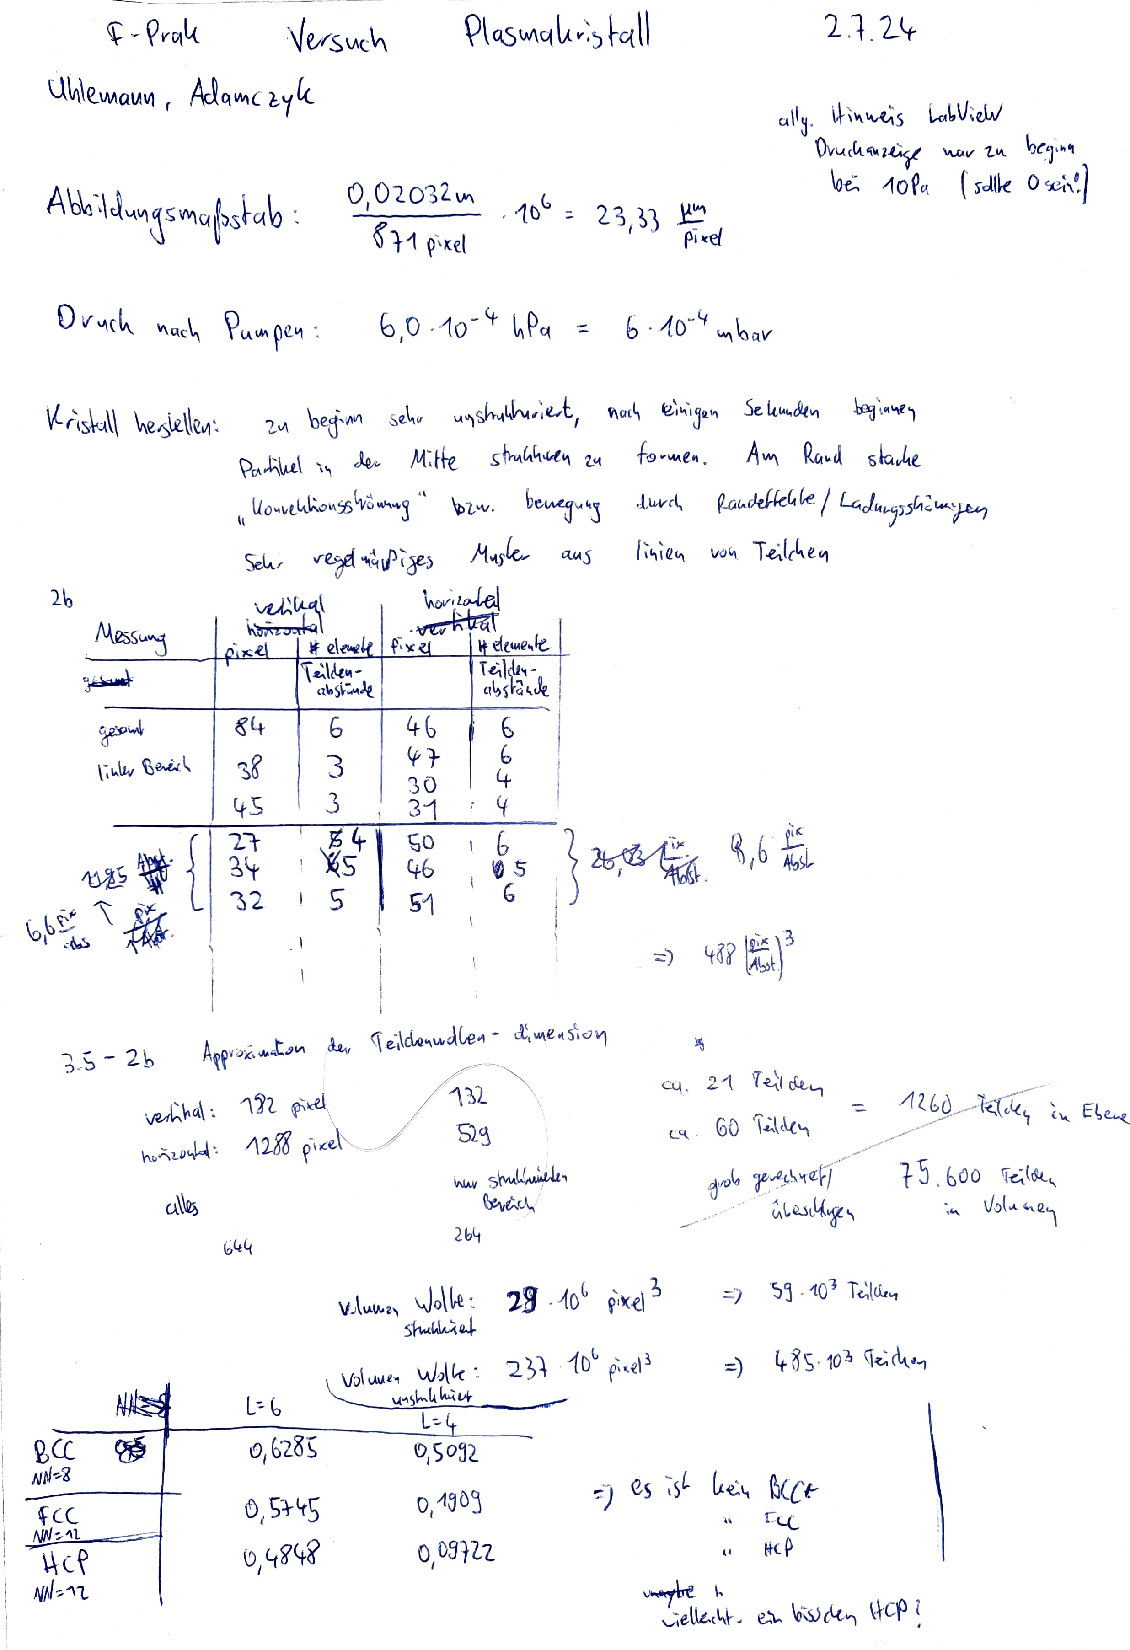
\includegraphics[width=0.95\textwidth, page=1]{data/Testat_Plasmakristall.pdf}		
	\caption[Testat 1]{Die erste Seite des Testats des Versuchs}
	\label{fig:Testat}
\end{figure}

\begin{figure}[ht]
	\centering
	\includegraphics[width=0.95\textwidth, page=2]{data/Testat_Plasmakristall.pdf}		
	\caption[Testat 2]{Die zweite Seite des Testats des Versuchs}
	\label{fig:Testat}
\end{figure}

\end{document}
